\subsection{Averages}
If we could deal with time series of infinite length, the distributions for a given system would be exactly the same.
This leads to the conclusion that other quantities like mean values or averages are more appropriate to describe the properties of such systems than their time series.
\paragraph{Time Average}
It is usually denoted by a bar $\bar{\ldots}$ over the quantity to be
averaged and calculated simply as the mean of a time series
\begin{equation}
	\bar{q}=\frac{1}{T}\int_0^T q(t)dt
\end{equation}
\paragraph{Ensemble Average}
It is usually denoted by brackets $\langle \ldots\rangle$ around the quantity, is calculated as the mean of the values from different realizations $k$ at the same point in time
\begin{equation}
	\langle q(t)\rangle=\frac{1}{N}\sum_{k=1}^N q_k(t)
\end{equation}
For so-called \textbf{Ergodic Systems\footnote{Ergodicity is a complicated matter. Roughly, a system is ergodic when its trajectory comes infinitely close to every point in phase space compatible with the system’s energy. All system we are talking about here are ergodic.}} the time and the ensemble average is the same $\bar{q}=\langle q(t)\rangle$.
Evidently, in this case the ensemble average is the same for all points in time.
\subsection{Distributions}
One of the main characteristics of a stochastic system is its \emph{probability distribution}.
The most common distribution, which is implemented in random number generators, is the \textbf{rectangular distribution}, where real numbers between 0 and 1 are drawn, all with the \emph{same probability}.
\subsubsection{Gaussian distribution}
It is given by
\begin{equation}
	g(x)=\frac{1}{\sigma\sqrt{2\pi}}e^{-\dfrac{(x-\mu)^2}{2\sigma^2}}\quad\text{with}\quad\int_{-\infty}^\infty g(x)\mathop{dx}=1
\end{equation}
where $\mu$ is the \emph{mean} and $\sigma$ the \emph{standard deviation}.
\paragraph{Properties of the Gaussian Distribution}
\begin{itemize}
	\item In very many cases the distributions found in nature are approximately Gaussian;
	\item It is a nontrivial distribution for which analytical results can be obtained.
\end{itemize}
The main reason for the first is that the sum of many independent stochastic variables has a Gaussian distribution whatever the individual distributions are.
More precisely, if the numbers $x_k$ are from independent stochastic processes then the variable
\begin{equation}
S_n=x_1+x_2+x_3+\cdots+x_n
\end{equation}
has a Gaussian distribution if $n$ goes to infinity independent of the distributions of the individual variables. This is the essence of the \textbf{central limit theorem}.\\
The second point has to do with a special property of the Gauss-function and what is known as the \emph{moments of a distribution}.
The $n_{th}$ moment $q(n)$ of a distribution $f(q)$ is define as
\begin{equation}
	q^{(n)}=\int_{-\infty}^\infty q^n f(q)\mathop{dq}
\end{equation}
This may look a little complicated but it is simply an extension of elementary statistics: the zeroth moment of any properly normalized distribution is 1 because it is just the integral over the distribution itself and the first moment is the mean value
\begin{equation}
	q^{(0)}=\int_{-\infty}^\infty f(q)\mathop{dq}=1\qquad q^{(1)}=\int_{-\infty}^\infty qf(q)\mathop{dq}=\langle q\rangle
\end{equation}
For $n>1$ it is more convenient to use the \emph{central moments} defined as
\begin{equation}
	\mu^{(n)}=\int_{-\infty}^\infty (q-\langle q\rangle)^n f(q)\mathop{dq}
\end{equation}
because the second central moment is the \emph{variance} with its square root the \emph{standard deviation}.
The third central moment defines the \emph{skewness} and the fourth the \emph{kurtosis} and so on.
\subsection{Correlations}
Besides distributions the second important property of a stochastic system is how fast (on average) it ‘forgets’ about its past, more precisely, how fast the \emph{correlations} within its time series decay.
A quantitative measure of correlation is the \emph{autocorrelation function}.\\
Imagine a time series $q(t)$ and a second time series, which is the same as the first, just shifted by a time $\tau$, $q(t-\tau)$, the autocorrelation function is defined as
\begin{equation}
	G(\tau)=\lim_{T\rightarrow\infty}\frac{\int\limits_{-T}^T q(t-\tau)q(t)\mathop{dt}}{\int\limits_{-T}^T q^2(t)\mathop{dt}}
\end{equation}
There exists an important relation between the autocorrelation function $G(\tau)$ of a time series and its spectrum $S(\omega)$, known as the \textbf{Wiener-Khinchin theorem}.
It states that the spectrum of a time series $S(\omega)$ is the Fourier transform of the autocorrelation function $G(\tau)$ and the autocorrelation function is the inverse Fourier transform of the spectrum.
We now have a look at the spectra and autocorrelation functions for three important cases.
\subsubsection{Periodic Signal}
Figure (\ref{fig:psas}) shows the time series $q(t)$ (a cosine), its distribution $p(q)$ and spectrum $S(\omega)$.
\begin{figure}[H]
	\centering
	\begin{subfigure}{0.45\linewidth}
		\centering
		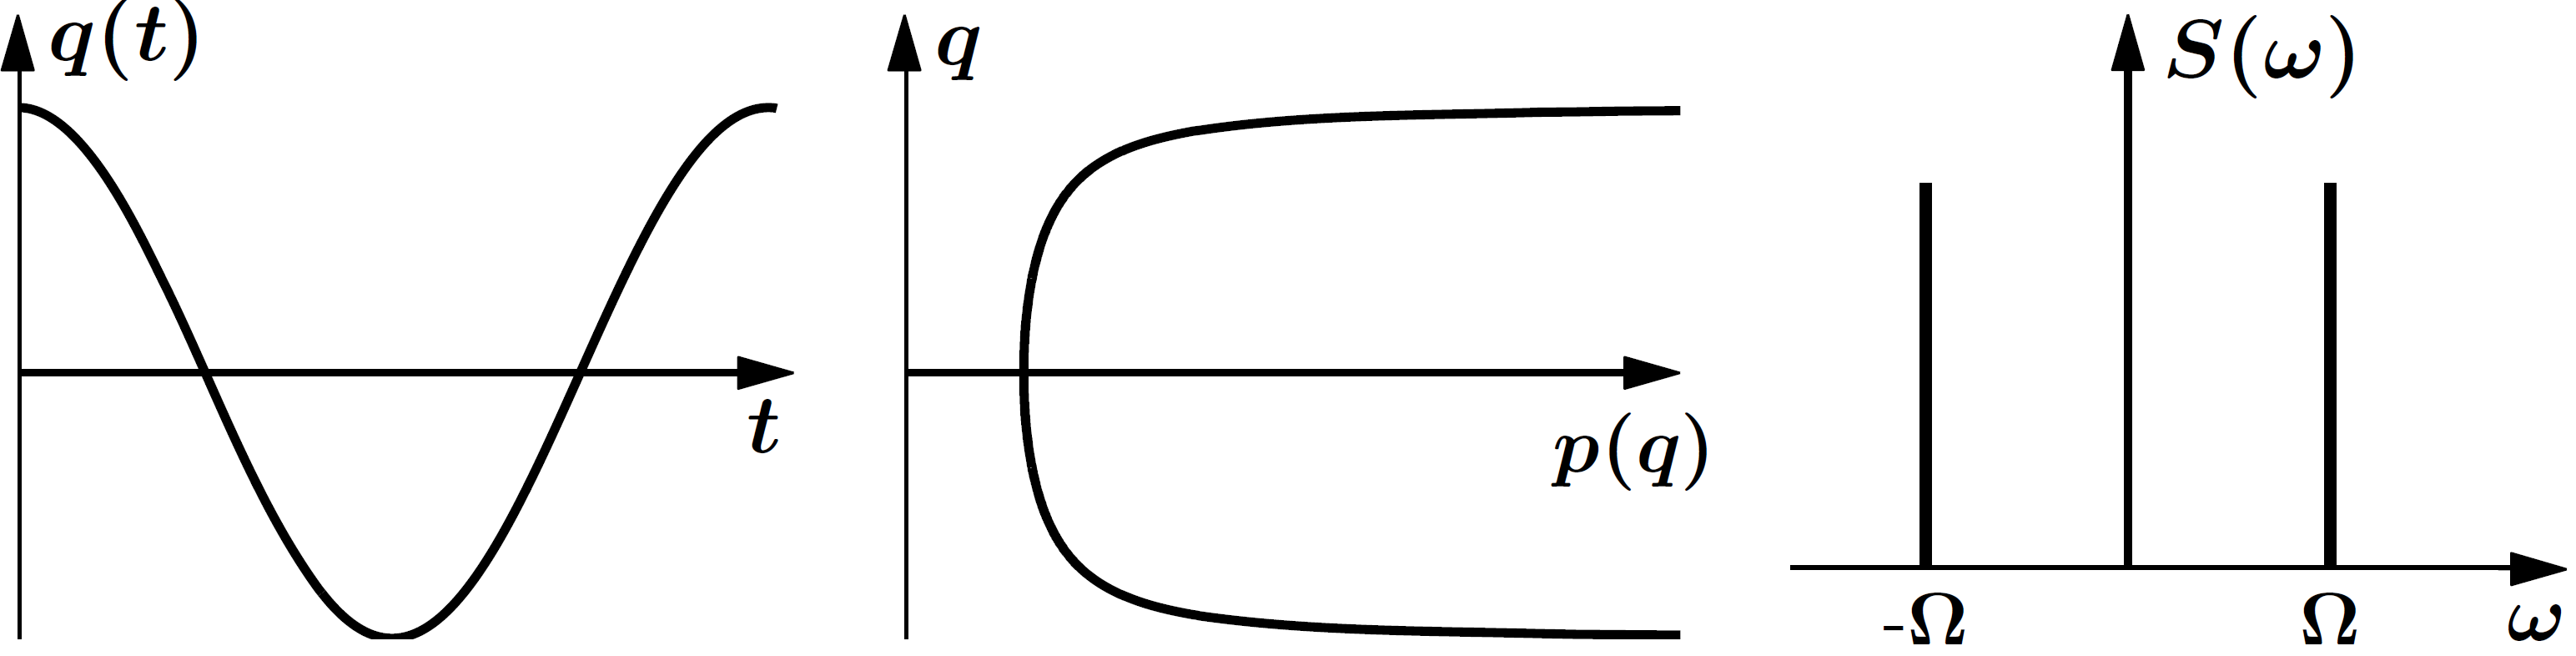
\includegraphics[width=\linewidth]{psas.png}
		\caption{Properties of a periodic signal.}
		\label{fig:psas}
	\end{subfigure}
	\vline
	\begin{subfigure}{0.45\linewidth}
		\centering
		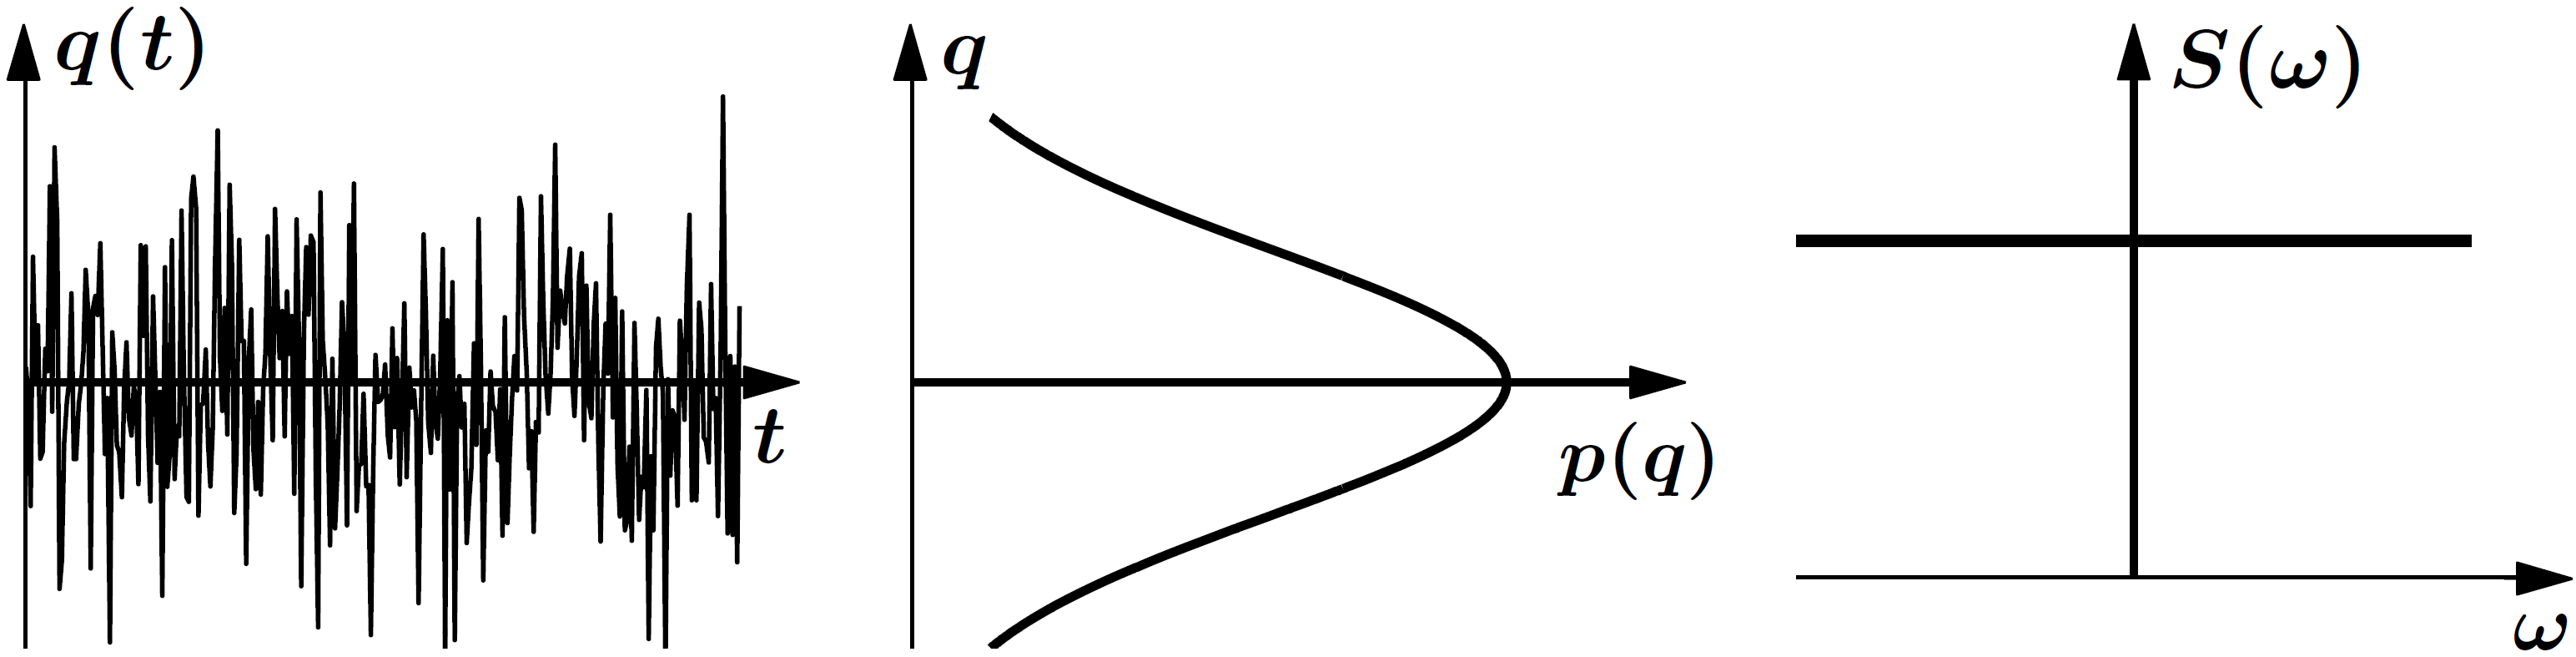
\includegraphics[width=\linewidth]{ucwnas.png}
		\caption{Properties of uncorrelated noise.}
		\label{fig:ucwnas}
	\end{subfigure}
	\caption{Left: Time series; middle: probability distribution; right: spectrum.}
\end{figure}
it can be shown that the distribution for the cosine function
\begin{equation}
	q(t)=\cos\Omega t\quad\text{is given by}\quad p(q)=\frac{1}{\sin\{\cosi q\}}
\end{equation}
We now calculate the autocorrelation function
\begin{equation}
	\begin{aligned}
		G(\tau)&=\lim_{T\rightarrow\infty}N\int_{-T}^T \cos\Omega(t-\tau)q(t)\mathop{dt}\quad\text{with the normalization factor}\quad\\
		G(\tau)&=\lim_{T\rightarrow\infty}\frac{N}{2}\int_{-T}^T\left\{\cos2\Omega(2t-\tau)+\cos\Omega\tau\right\}\mathop{dt}\\
		G(\tau)&=\cos\Omega \tau\quad\text{as}\quad T\rightarrow\infty\\
	\end{aligned}
	\begin{aligned}
		N&=\left\{\int_{-T}^T\cos^2\Omega t\mathop{dt}\right\}^{-1}\\
		\frac{1}{N}&=\frac{\cos\Omega T\sin\Omega T}{\Omega}+T\\
		N&\approx\frac{1}{T}\quad\text{as}\quad T\rightarrow\infty\\
	\end{aligned}
\end{equation}
So for a cosine the autocorrelation function does not simply decrease with an increasing shift but oscillates and has a value of 1 at all even multiples of $\frac{\pi}{\Omega}$, and a value of $-1$ (anti-correlated) at all odd multiples.
	In other words: for such a purely deterministic and periodic signal the correlation does not fall off in time and the \emph{correlation length} is infinite.
\subsubsection{Uncorrelated (white) Noise}
The most common representation for uncorrelated or white noise is of the form
\begin{equation}
	\langle \xi(t)\xi(t^\prime)\rangle=Q\delta(t-t^\prime)\quad\text{where}\quad Q=\text{noise strength}
\end{equation}
By writing $t^\prime$ in the form $t-\tau$ the average autocorrelation function takes the form
\begin{equation}
	\begin{aligned}
		\langle G(\tau)\rangle&=\langle \lim_{T\rightarrow\infty}N\int_{-T}^T \xi(t)\xi(t-\tau)\mathop{dt}\rangle\\
		&=\lim_{T\rightarrow\infty}\langle N\rangle\int_{-T}^T Q\delta\{t-(t-\tau)\}\mathop{dt}\\
		&=\lim_{T\rightarrow\infty}\langle N\rangle2TQ\delta(\tau)\\
		\langle G(\tau)\rangle&=\frac{\delta(\tau)}{\delta(0)}=
		\begin{cases}
			1&\text{if}\ \tau=0\\
			0&\text{if}\ \tau\neq0
		\end{cases}\\
	\end{aligned}\quad\text{with the normalization factor}\quad
	\begin{aligned}
		\langle N^{-1}\rangle&=\int_{-T}^T \langle \xi^2(t)\rangle\mathop{dt}\\
		&=\int_{-T}^T Q\delta(0)\mathop{dt}\\
		&=2TQ\delta(0)\\
	\end{aligned}
\end{equation}
It means that the time series is only correlated at the trivial point $\tau=0$ and the correlations vanish for any finite shift, so the correlation length is zero.\\
The features of uncorrelated noise, time series, probability distribution and spectrum are summarized in Figure (\ref{fig:ucwnas}).
\subsubsection{Noise with Finite Correlation Length}
Between the two extreme cases just discussed, correlation lengths of zero and infinity, there are stochastic systems with finite correlations like those where the autocorrelation function falls off exponentially with the shift $\tau$
\begin{equation}
	G(\tau)=e^{-\alpha|\tau|}\quad\text{where}\quad\frac{1}{\alpha}=t_c
\end{equation}
The correlation length, $t_c$, represents the time after which (on the average) the correlations have decreased by a factor of $e^{-1}$.
The spectrum for a stochastic process for which the correlations fall off exponentially in time
\begin{equation}
	S(\omega)=\frac{2\alpha}{\alpha^2+\omega^2}
\end{equation}
Figure (\ref{fig:psfcas}) shows an example of such functions.
They look like the Gaussians but are rational functions, not exponentials, and are called \textbf{Lorentzians}.
\begin{figure}[h!]
	\centering
	\begin{subfigure}{0.5\linewidth}
		\centering
		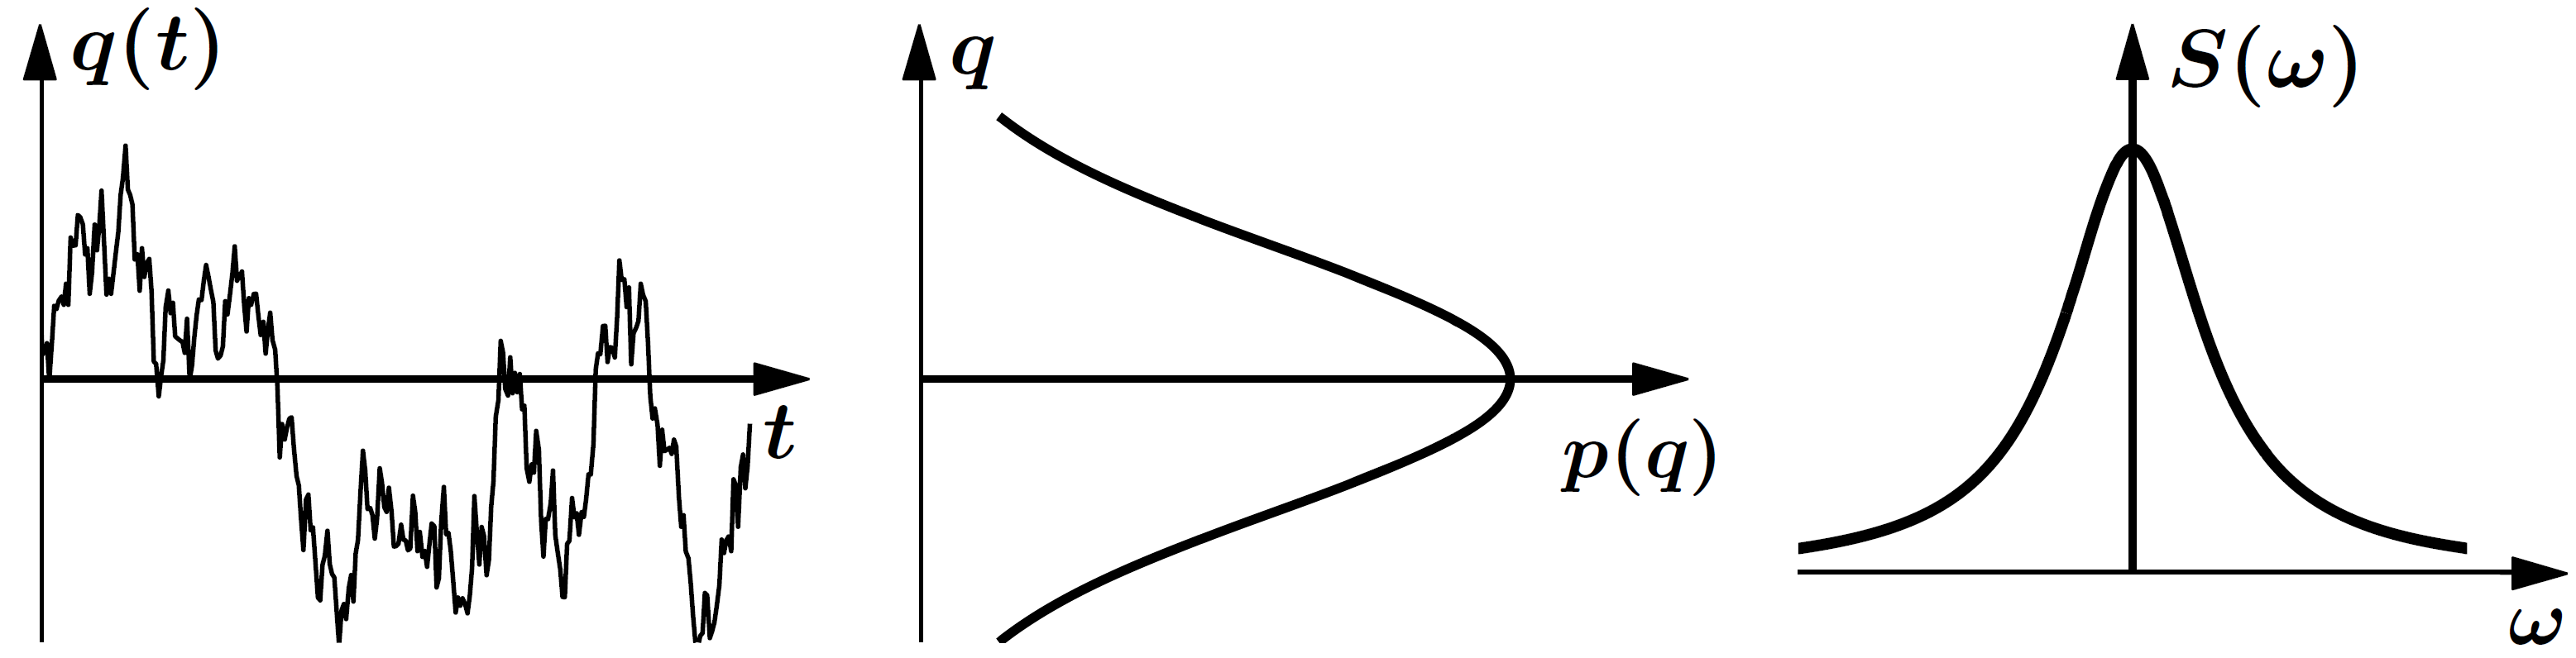
\includegraphics[width=\linewidth]{psfcas.png}
		\caption{Properties of a signal with finite correlations. Left: time series; middle: probability distribution; right: spectrum.}
		\label{fig:psfcas}
	\end{subfigure}
	\vline
	\begin{subfigure}{0.43\linewidth}
		\centering
		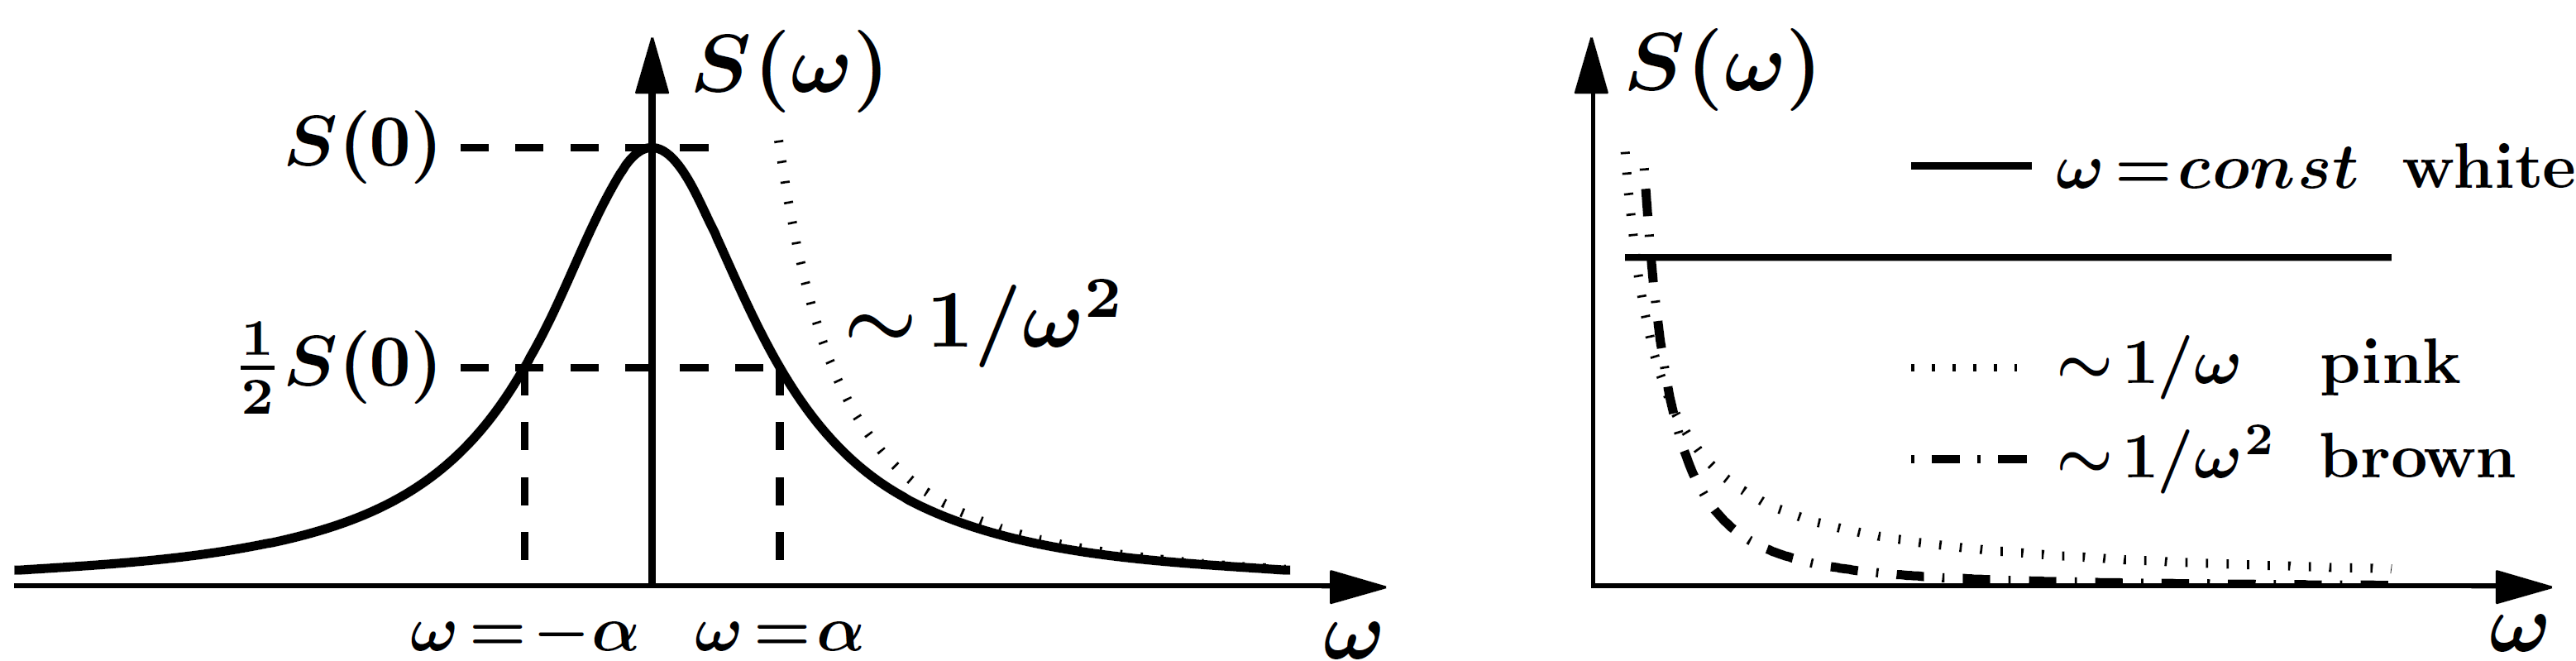
\includegraphics[width=\linewidth]{plas.png}
		\caption{Properties of the Lorentzian. Left:The function has half of its maximum value at $\omega=\alpha$ and falls off proportional to $w^2$. Right:The most important noise colors}
		\label{fig:plas}
	\end{subfigure}
\end{figure}
\subsubsection{Colors of Noise}
Certain types of stochastic time series can be classified according to their spectra and are associated with a ‘color’.\\
The most important color of noise is \textbf{white}: as for the corresponding white light, the spectrum is a constant, i.e. all frequencies have the same amplitude and, the correlation is a $\delta-$function.\\
A time series with a spectrum that for large values of $\omega$ it falls off proportional to $\omega^{-2}$ is called \textbf{brown} or \textbf{Brownian noise}.\\
A further property of these two noise types is that white noise is the \emph{derivative} of brown noise and, accordingly, brown noise is the \emph{integral} of white noise in time.\\
In between is a noise type known as \textbf{pink}, whose spectrum falls of proportional to $\omega^{-1}$.\\
Spectra for white, pink and brown noise are shown in Figure (\ref{fig:plas}(right)).